%%
%% GAC: When Smaller Is Slower — Dimensional Collapse in Compressed LLMs
%% Target: EuroMLSys 2026 (SIGPLAN format, 6 pages excluding references)
%%

\documentclass[sigplan,10pt,nonacm]{acmart}

%% Remove ACM-specific elements for submission
\settopmatter{printacmref=false,authorsperrow=5}
\renewcommand\footnotetextcopyrightpermission[1]{}
\pagestyle{plain}

%% Packages
\usepackage{booktabs}
\usepackage{subcaption}
\usepackage{listings}
\usepackage{xcolor}
\usepackage{graphicx}
\usepackage{tikz}
\usetikzlibrary{positioning,decorations.pathreplacing}
\usepackage{placeins}
\usepackage{colortbl}
\usepackage{seqsplit}

%% Code listing style
\lstset{
  basicstyle=\ttfamily\small,
  breaklines=true,
  frame=single,
  numbers=left,
  numberstyle=\tiny,
}

%% Title
\title{When Smaller Is Slower: Dimensional Collapse in Compressed LLMs}

%% Authors
\author{Jihao Xin}
\affiliation{
  \institution{KAUST}
  \country{Saudi Arabia}
}

\author{Tian Lvy}
\affiliation{
  \institution{KAUST}
  \country{Saudi Arabia}
}

\author{Qilong Pan}
\affiliation{
  \institution{HUMAIN AI}
  \country{Saudi Arabia}
}

\author{Kesen Wang}
\affiliation{
  \institution{HUMAIN AI}
  \country{Saudi Arabia}
}

\author{Marco Canini}
\affiliation{
  \institution{KAUST}
  \country{Saudi Arabia}
}

\begin{abstract}
Post-training compression can produce irregular tensor dimensions that cause GPU slowdowns despite reducing FLOPs---a phenomenon we term \emph{dimensional collapse}.
We systematically diagnose three root causes on NVIDIA A100: Tensor Core misalignment (58\%), vectorized load degradation (50\%), and SDPA bandwidth inefficiency (40\%).
We then propose \textbf{GAC} (GPU-Aligned Compression), a multi-choice knapsack algorithm that selects aligned rank allocations during compression.
On Llama-3-8B with SVD compression (ratio 0.7), GAC achieves the best perplexity (14.30) among all allocation strategies at the same parameter budget, while guaranteeing 100\% dimension alignment---compared to unconstrained allocation which leaves 41\% of dimensions misaligned with 10.4\% latency overhead and worse perplexity (14.44).
For existing compressed models, post-hoc dimension repair recovers 22--28\% kernel speedup with 3.7\% memory overhead.
\end{abstract}

\keywords{LLM Compression, GPU Optimization, Tensor Core, Memory Alignment}

\begin{document}

\maketitle


%% ===========================================
%% 1. INTRODUCTION
%% ===========================================
\section{Introduction}
\label{sec:intro}

Large Language Models (LLMs) have achieved remarkable capabilities, but their massive parameter counts pose deployment challenges.
Post-training compression---pruning, low-rank decomposition, token eviction---offers promising solutions.
However, these techniques often produce \emph{irregular tensor dimensions} that do not align with hardware-preferred multiples (8, 16, 32).

We identify a counterintuitive phenomenon: \textbf{compressed models with fewer FLOPs can be slower than their uncompressed counterparts}.
We term this \emph{dimensional collapse}---nonlinear performance degradation caused by misalignment between software-defined tensor shapes and hardware-fixed access patterns.
Formally, a dimension $d$ is \emph{misaligned} when $d \bmod 8 \neq 0$ and \emph{aligned} otherwise.

\paragraph{Motivating Example.}
Importance-based SVD rank allocation for Llama-3-8B produces ranks like 107 instead of 112.
On A100, GEMM with $K$=107 is 30\% slower than $K$=112 (same kernel tier); SDPA latency increases 88\% ($d$=107 vs $d$=96).
Across four scoring methods, 43--91\% of unconstrained SVD ranks are misaligned.

\paragraph{Three pathways to dimensional collapse.}
Different compression techniques alter different GEMM dimensions:
\textbf{(i)} SVD/low-rank decomposition changes the $K$ dimension (inner rank);
\textbf{(ii)} pruning changes the $N$ dimension (output features);
\textbf{(iii)} token eviction changes the $M$ dimension (sequence length).
Each pathway has distinct alignment sensitivities (\S\ref{sec:analysis}).

\paragraph{Scope.}
Our analysis targets compression methods \emph{without} built-in alignment constraints (vanilla SVD, Fisher-weighted SVD~\cite{fwsvd2022,gfwsvd2025}).
Production PaLU~\cite{palu} enforces 32-multiple alignment internally; our work explains \emph{why} this is necessary and provides a principled algorithm to do it optimally.

% fig1_overview.tex — Dimensional Collapse Overview (TikZ)
% Usage: % fig1_overview.tex — Dimensional Collapse Overview (TikZ)
% Usage: % fig1_overview.tex — Dimensional Collapse Overview (TikZ)
% Usage: \input{figures/fig1_overview.tex}
\begin{figure*}[t]
\centering
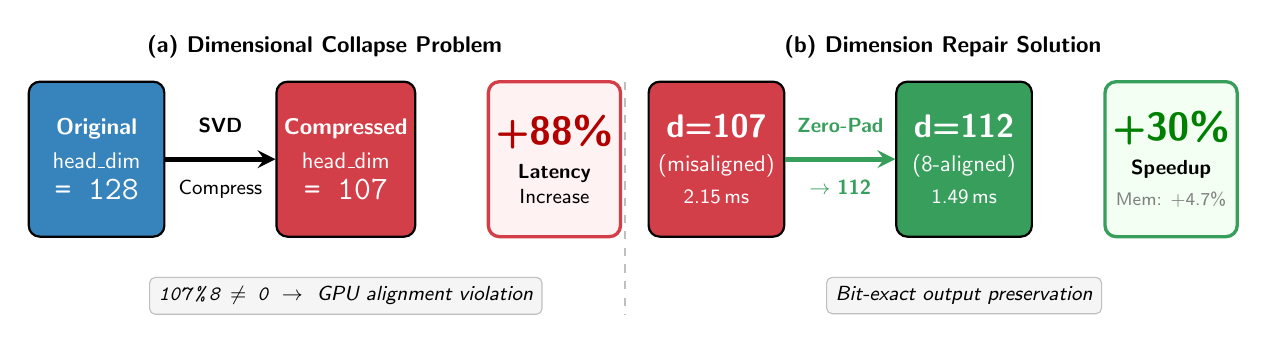
\begin{tikzpicture}[scale=0.82, every node/.style={scale=0.82},
    >=stealth,
    node distance=1.2cm,
    box/.style={
      draw, rounded corners=4pt, minimum width=2.1cm, minimum height=2.4cm,
      line width=0.8pt, text=white, font=\sffamily, align=center
    },
    metric/.style={
      draw, rounded corners=4pt, minimum width=1.9cm, minimum height=2.4cm,
      line width=1.2pt, align=center, font=\sffamily
    },
    lbl/.style={font=\sffamily\small, align=center},
    note/.style={font=\sffamily\small\itshape, fill=gray!8, draw=gray!50,
                 rounded corners=2pt, inner sep=4pt}
  ]

  % ===== (a) Left panel: Dimensional Collapse Problem =====
  \begin{scope}[local bounding box=panelA]
    % Original model
    \node[box, fill={rgb,255:red,55;green,131;blue,187}] (orig) {
      \textbf{\normalsize Original}\\[3pt]
      head\_dim\\[2pt]
      {\Large\bfseries\ttfamily = 128}
    };

    % Arrow: SVD compress
    \node[box, fill={rgb,255:red,211;green,63;blue,73}, right=1.4cm of orig] (comp) {
      \textbf{\normalsize Compressed}\\[3pt]
      head\_dim\\[2pt]
      {\Large\bfseries\ttfamily = 107}
    };
    \draw[->, line width=1.8pt] (orig.east) -- (comp.west)
      node[midway, above=6pt, lbl] {\textbf{SVD}}
      node[midway, below=4pt, lbl] {Compress};

    % Impact metric
    \node[metric, fill=red!5, draw={rgb,255:red,211;green,63;blue,73},
          right=0.9cm of comp] (impact) {
      {\color{red!70!black}\fontsize{18}{20}\selectfont\bfseries +88\%}\\[3pt]
      {\small\bfseries Latency}\\[-1pt]
      {\small Increase}
    };

    % Bottom note
    \node[note, below=0.5cm of comp]
      {{\ttfamily 107\,\%\,8 $\neq$ 0} ~$\to$~ GPU alignment violation};
  \end{scope}

  % Panel (a) title
  \node[above=0.2cm of panelA.north, font=\sffamily\bfseries] {(a) Dimensional Collapse Problem};

  % ===== (b) Right panel: Dimension Repair Solution =====
  \begin{scope}[xshift=9.6cm, local bounding box=panelB]
    % Misaligned input
    \node[box, fill={rgb,255:red,211;green,63;blue,73}] (mis) {
      {\Large\bfseries d=107}\\[3pt]
      (misaligned)\\[2pt]
      {\small 2.15\,ms}
    };

    % Repaired output
    \node[box, fill={rgb,255:red,56;green,158;blue,92}, right=1.4cm of mis] (rep) {
      {\Large\bfseries d=112}\\[3pt]
      (8-aligned)\\[2pt]
      {\small 1.49\,ms}
    };
    \draw[->, line width=1.8pt, color={rgb,255:red,56;green,158;blue,92}]
      (mis.east) -- (rep.west)
      node[midway, above=6pt, lbl, text={rgb,255:red,56;green,158;blue,92}] {\textbf{Zero-Pad}}
      node[midway, below=4pt, lbl, text={rgb,255:red,56;green,158;blue,92}] {$\to$ \textbf{112}};

    % Result metric
    \node[metric, fill=green!5, draw={rgb,255:red,56;green,158;blue,92},
          right=0.9cm of rep] (result) {
      {\color{green!50!black}\fontsize{18}{20}\selectfont\bfseries +30\%}\\[3pt]
      {\small\bfseries Speedup}\\[2pt]
      {\footnotesize\color{gray} Mem: +4.7\%}
    };

    % Bottom note
    \node[note, below=0.5cm of rep]
      {Bit-exact output preservation};
  \end{scope}

  % Panel (b) title
  \node[above=0.2cm of panelB.north, font=\sffamily\bfseries] {(b) Dimension Repair Solution};

  % Dashed separator between panels
  \draw[dashed, gray!50, line width=0.5pt]
    ([xshift=4.65cm]panelA.north) -- ([xshift=4.65cm]panelA.south);

\end{tikzpicture}
\caption{\textbf{Dimensional collapse overview.} (a)~Unconstrained SVD compression produces irregular dimensions. Across four importance scoring methods and all projection matrices, 43--91\% of dimensions would be misaligned, triggering GPU performance cliffs via Tensor Core and memory alignment violations. (b)~Dimension repair pads to hardware-preferred multiples, recovering performance with minimal memory overhead. See \S\ref{sec:distribution} for distribution analysis and \S\ref{sec:root_cause} for root causes.}
\label{fig:overview}
\end{figure*}

\begin{figure*}[t]
\centering
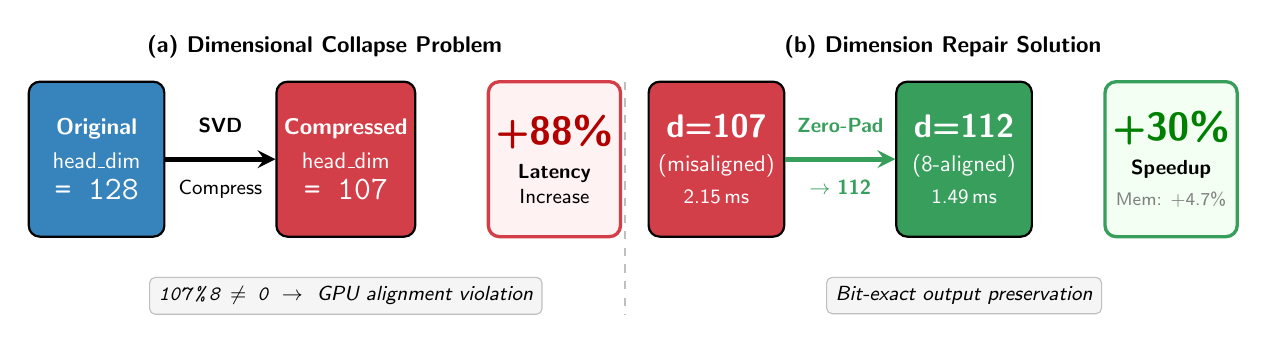
\begin{tikzpicture}[scale=0.82, every node/.style={scale=0.82},
    >=stealth,
    node distance=1.2cm,
    box/.style={
      draw, rounded corners=4pt, minimum width=2.1cm, minimum height=2.4cm,
      line width=0.8pt, text=white, font=\sffamily, align=center
    },
    metric/.style={
      draw, rounded corners=4pt, minimum width=1.9cm, minimum height=2.4cm,
      line width=1.2pt, align=center, font=\sffamily
    },
    lbl/.style={font=\sffamily\small, align=center},
    note/.style={font=\sffamily\small\itshape, fill=gray!8, draw=gray!50,
                 rounded corners=2pt, inner sep=4pt}
  ]

  % ===== (a) Left panel: Dimensional Collapse Problem =====
  \begin{scope}[local bounding box=panelA]
    % Original model
    \node[box, fill={rgb,255:red,55;green,131;blue,187}] (orig) {
      \textbf{\normalsize Original}\\[3pt]
      head\_dim\\[2pt]
      {\Large\bfseries\ttfamily = 128}
    };

    % Arrow: SVD compress
    \node[box, fill={rgb,255:red,211;green,63;blue,73}, right=1.4cm of orig] (comp) {
      \textbf{\normalsize Compressed}\\[3pt]
      head\_dim\\[2pt]
      {\Large\bfseries\ttfamily = 107}
    };
    \draw[->, line width=1.8pt] (orig.east) -- (comp.west)
      node[midway, above=6pt, lbl] {\textbf{SVD}}
      node[midway, below=4pt, lbl] {Compress};

    % Impact metric
    \node[metric, fill=red!5, draw={rgb,255:red,211;green,63;blue,73},
          right=0.9cm of comp] (impact) {
      {\color{red!70!black}\fontsize{18}{20}\selectfont\bfseries +88\%}\\[3pt]
      {\small\bfseries Latency}\\[-1pt]
      {\small Increase}
    };

    % Bottom note
    \node[note, below=0.5cm of comp]
      {{\ttfamily 107\,\%\,8 $\neq$ 0} ~$\to$~ GPU alignment violation};
  \end{scope}

  % Panel (a) title
  \node[above=0.2cm of panelA.north, font=\sffamily\bfseries] {(a) Dimensional Collapse Problem};

  % ===== (b) Right panel: Dimension Repair Solution =====
  \begin{scope}[xshift=9.6cm, local bounding box=panelB]
    % Misaligned input
    \node[box, fill={rgb,255:red,211;green,63;blue,73}] (mis) {
      {\Large\bfseries d=107}\\[3pt]
      (misaligned)\\[2pt]
      {\small 2.15\,ms}
    };

    % Repaired output
    \node[box, fill={rgb,255:red,56;green,158;blue,92}, right=1.4cm of mis] (rep) {
      {\Large\bfseries d=112}\\[3pt]
      (8-aligned)\\[2pt]
      {\small 1.49\,ms}
    };
    \draw[->, line width=1.8pt, color={rgb,255:red,56;green,158;blue,92}]
      (mis.east) -- (rep.west)
      node[midway, above=6pt, lbl, text={rgb,255:red,56;green,158;blue,92}] {\textbf{Zero-Pad}}
      node[midway, below=4pt, lbl, text={rgb,255:red,56;green,158;blue,92}] {$\to$ \textbf{112}};

    % Result metric
    \node[metric, fill=green!5, draw={rgb,255:red,56;green,158;blue,92},
          right=0.9cm of rep] (result) {
      {\color{green!50!black}\fontsize{18}{20}\selectfont\bfseries +30\%}\\[3pt]
      {\small\bfseries Speedup}\\[2pt]
      {\footnotesize\color{gray} Mem: +4.7\%}
    };

    % Bottom note
    \node[note, below=0.5cm of rep]
      {Bit-exact output preservation};
  \end{scope}

  % Panel (b) title
  \node[above=0.2cm of panelB.north, font=\sffamily\bfseries] {(b) Dimension Repair Solution};

  % Dashed separator between panels
  \draw[dashed, gray!50, line width=0.5pt]
    ([xshift=4.65cm]panelA.north) -- ([xshift=4.65cm]panelA.south);

\end{tikzpicture}
\caption{\textbf{Dimensional collapse overview.} (a)~Unconstrained SVD compression produces irregular dimensions. Across four importance scoring methods and all projection matrices, 43--91\% of dimensions would be misaligned, triggering GPU performance cliffs via Tensor Core and memory alignment violations. (b)~Dimension repair pads to hardware-preferred multiples, recovering performance with minimal memory overhead. See \S\ref{sec:distribution} for distribution analysis and \S\ref{sec:root_cause} for root causes.}
\label{fig:overview}
\end{figure*}

\begin{figure*}[t]
\centering
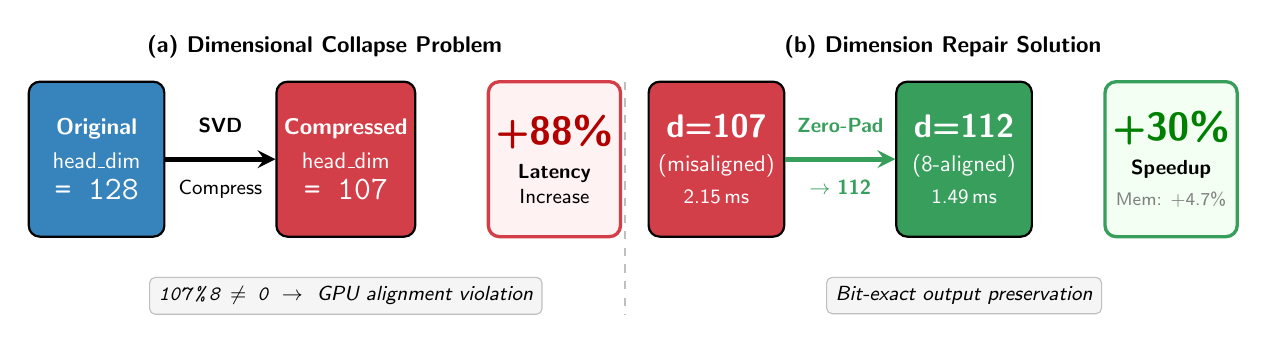
\begin{tikzpicture}[scale=0.82, every node/.style={scale=0.82},
    >=stealth,
    node distance=1.2cm,
    box/.style={
      draw, rounded corners=4pt, minimum width=2.1cm, minimum height=2.4cm,
      line width=0.8pt, text=white, font=\sffamily, align=center
    },
    metric/.style={
      draw, rounded corners=4pt, minimum width=1.9cm, minimum height=2.4cm,
      line width=1.2pt, align=center, font=\sffamily
    },
    lbl/.style={font=\sffamily\small, align=center},
    note/.style={font=\sffamily\small\itshape, fill=gray!8, draw=gray!50,
                 rounded corners=2pt, inner sep=4pt}
  ]

  % ===== (a) Left panel: Dimensional Collapse Problem =====
  \begin{scope}[local bounding box=panelA]
    % Original model
    \node[box, fill={rgb,255:red,55;green,131;blue,187}] (orig) {
      \textbf{\normalsize Original}\\[3pt]
      head\_dim\\[2pt]
      {\Large\bfseries\ttfamily = 128}
    };

    % Arrow: SVD compress
    \node[box, fill={rgb,255:red,211;green,63;blue,73}, right=1.4cm of orig] (comp) {
      \textbf{\normalsize Compressed}\\[3pt]
      head\_dim\\[2pt]
      {\Large\bfseries\ttfamily = 107}
    };
    \draw[->, line width=1.8pt] (orig.east) -- (comp.west)
      node[midway, above=6pt, lbl] {\textbf{SVD}}
      node[midway, below=4pt, lbl] {Compress};

    % Impact metric
    \node[metric, fill=red!5, draw={rgb,255:red,211;green,63;blue,73},
          right=0.9cm of comp] (impact) {
      {\color{red!70!black}\fontsize{18}{20}\selectfont\bfseries +88\%}\\[3pt]
      {\small\bfseries Latency}\\[-1pt]
      {\small Increase}
    };

    % Bottom note
    \node[note, below=0.5cm of comp]
      {{\ttfamily 107\,\%\,8 $\neq$ 0} ~$\to$~ GPU alignment violation};
  \end{scope}

  % Panel (a) title
  \node[above=0.2cm of panelA.north, font=\sffamily\bfseries] {(a) Dimensional Collapse Problem};

  % ===== (b) Right panel: Dimension Repair Solution =====
  \begin{scope}[xshift=9.6cm, local bounding box=panelB]
    % Misaligned input
    \node[box, fill={rgb,255:red,211;green,63;blue,73}] (mis) {
      {\Large\bfseries d=107}\\[3pt]
      (misaligned)\\[2pt]
      {\small 2.15\,ms}
    };

    % Repaired output
    \node[box, fill={rgb,255:red,56;green,158;blue,92}, right=1.4cm of mis] (rep) {
      {\Large\bfseries d=112}\\[3pt]
      (8-aligned)\\[2pt]
      {\small 1.49\,ms}
    };
    \draw[->, line width=1.8pt, color={rgb,255:red,56;green,158;blue,92}]
      (mis.east) -- (rep.west)
      node[midway, above=6pt, lbl, text={rgb,255:red,56;green,158;blue,92}] {\textbf{Zero-Pad}}
      node[midway, below=4pt, lbl, text={rgb,255:red,56;green,158;blue,92}] {$\to$ \textbf{112}};

    % Result metric
    \node[metric, fill=green!5, draw={rgb,255:red,56;green,158;blue,92},
          right=0.9cm of rep] (result) {
      {\color{green!50!black}\fontsize{18}{20}\selectfont\bfseries +30\%}\\[3pt]
      {\small\bfseries Speedup}\\[2pt]
      {\footnotesize\color{gray} Mem: +4.7\%}
    };

    % Bottom note
    \node[note, below=0.5cm of rep]
      {Bit-exact output preservation};
  \end{scope}

  % Panel (b) title
  \node[above=0.2cm of panelB.north, font=\sffamily\bfseries] {(b) Dimension Repair Solution};

  % Dashed separator between panels
  \draw[dashed, gray!50, line width=0.5pt]
    ([xshift=4.65cm]panelA.north) -- ([xshift=4.65cm]panelA.south);

\end{tikzpicture}
\caption{\textbf{Dimensional collapse overview.} (a)~Unconstrained SVD compression produces irregular dimensions. Across four importance scoring methods and all projection matrices, 43--91\% of dimensions would be misaligned, triggering GPU performance cliffs via Tensor Core and memory alignment violations. (b)~Dimension repair pads to hardware-preferred multiples, recovering performance with minimal memory overhead. See \S\ref{sec:distribution} for distribution analysis and \S\ref{sec:root_cause} for root causes.}
\label{fig:overview}
\end{figure*}


\paragraph{Contributions.}
\textbf{(1)}~Systematic quantification of dimensional collapse across GEMM and SDPA, identifying three confirmed root causes (\S\ref{sec:analysis}).
\textbf{(2)}~\textbf{GAC}: a multi-choice knapsack DP algorithm for alignment-aware rank allocation that achieves Pareto dominance---better accuracy \emph{and} alignment than naive rounding (\S\ref{sec:gac}).
\textbf{(3)}~End-to-end validation on Llama-3-8B: GAC achieves the best perplexity (14.30) among SVD-only methods at the same parameter budget, with 100\% alignment (\S\ref{sec:eval}).
\textbf{(4)}~Post-hoc dimension repair for existing models: 22--28\% kernel speedup, 3.7\% memory overhead (\S\ref{sec:eval}).


%% ===========================================
%% 2. BACKGROUND
%% ===========================================
\section{Background}
\label{sec:background}

\paragraph{Tensor Core Alignment.}
NVIDIA Tensor Cores perform MMA on fixed tile sizes~\cite{nvidia_perf_guide}.
For FP16 on A100, optimal operation requires $K \bmod 16 = 0$.
Misaligned dimensions force padding or fallback to slower paths.

\paragraph{SDPA Backends.}
PyTorch SDPA~\cite{pytorch_sdpa} dispatches to three backends: FlashAttention-2~\cite{flashattention2}, MEM\_EFFICIENT, and MATH.
FlashAttention-2 selects the smallest template $\geq d$ from $\{64, 96, 128, 160, 192, 224, 256\}$, with tile configuration $(B_r \times B_c)$ decreasing at each boundary---directly affecting iteration count and latency (\S\ref{sec:sdpa}).
MEM\_EFFICIENT requires $d \bmod 8 = 0$; when unavailable, PyTorch falls back to MATH (12$\times$ slower).

\paragraph{Low-Rank Compression.}
SVD-based methods~\cite{palu,svdllm2024} decompose $W \approx U_r \Sigma_r V_r^T$, where $r$ is the per-layer rank.
Importance-based allocation distributes ranks proportionally to layer sensitivity (Fisher information, magnitude)~\cite{fwsvd2022,gfwsvd2025}, typically producing non-aligned values.


%% ===========================================
%% 3. ANALYSIS: DIMENSIONAL COLLAPSE
%% ===========================================
\section{Analysis: Dimensional Collapse}
\label{sec:analysis}

All experiments run on NVIDIA A100-80GB (PyTorch 2.9.1, CUDA 12.8, FP16). Latency uses CUDA event timing (warmup=50, measure=200, 3 trials).

\subsection{Dimension Distribution in Practice}
\label{sec:distribution}

To quantify how common misalignment is, we analyze unconstrained SVD rank allocation for Llama-3-8B ($r$=0.8) using four importance scoring methods (Fisher, magnitude, activation, gradient) across all K/V/Q/O projections (Figure~\ref{fig:dim_scatter} in Appendix~\ref{app:scatter}).
Results: 43--91\% of dimensions are not 8-aligned (average 70.5\% across all 16 method$\times$projection combinations).
RAP SVD~\cite{rap} produces 100\% misaligned dimensions ($d$=102 for $r$=0.8).
This confirms that misalignment is a \emph{structural property} of unconstrained importance-based allocation, not an edge case.
Production PaLU~\cite{palu} avoids this by enforcing 32-multiple alignment internally---but at the cost of suboptimal rank distribution (weighted deviation 5$\times$ higher than GAC, Table~\ref{tab:gac}).

\subsection{GEMM Alignment Sensitivity}
\label{sec:gemm}

We sweep each GEMM dimension independently while fixing the others at typical LLM sizes ($M$=2048, $N$=2048, $K$=128).
Figure~\ref{fig:gemm_alignment} shows the results.

\begin{figure*}[t]
\centering
\includegraphics[width=\textwidth]{figures/fig_gemm_alignment.pdf}
\caption{\textbf{GEMM alignment sensitivity.} Latency vs.\ dimension value for $M$ (token count, 1024--2048), $N$ (pruning, 1024--2048), $K$ (SVD rank, 64--128). Pink fill shows the alignment penalty: misaligned values ($d$ mod $8 \neq 0$) consistently incur higher latency. $M$ and $N$ panels also show cuBLAS kernel switching points (A/B/C denote kernel families with different CTA tile sizes; see \S\ref{sec:kernel_tier}).}
\label{fig:gemm_alignment}
\end{figure*}

\paragraph{$K$ dimension (SVD rank).}
The $K$ panel shows a clean alignment effect: aligned values ($K$ mod $8 = 0$) achieve $\sim$20\,$\mu$s while misaligned values reach 22--26\,$\mu$s (up to 30\% penalty).
This directly impacts low-rank compression methods.

\paragraph{$N$ dimension (pruning).}
$N$ shows similar alignment sensitivity to $K$, plus kernel-switching cliffs where cuBLAS transitions between kernel families (Figure~\ref{fig:gemm_alignment}b, labels B$\to$C at $N$$\approx$1250 and C$\to$B at $N$$\approx$1664).
Misaligned $N$ values trigger CUTLASS align1/align2 kernels instead of cuBLAS-native sm80 kernels.

\paragraph{$M$ dimension (token eviction).}
$M$ is insensitive to mod-8 alignment---both aligned and misaligned values use similar kernels at a given range.
However, it exhibits staircase effects from cuBLAS heuristic kernel selection: $M$=1728$\to$1729 triggers a transition from hand-tuned SASS kernel (CTA 256$\times$128) to XMMA codegen kernel (CTA 192$\times$128), reducing SM utilization from 100\% to 48\% and increasing latency by $\sim$30\%.
This demonstrates that dimensional collapse extends beyond alignment: even aligned dimensions can hit performance cliffs from kernel heuristic boundaries.

\subsection{SDPA Latency}
\label{sec:sdpa}

We sweep \texttt{head\_dim} from 64 to 256 ($B$=4, $S$=2048, $H$=32).
Figure~\ref{fig:sdpa_latency} reveals a pronounced \emph{staircase} pattern driven by FlashAttention-2's template selection mechanism.

\paragraph{FA2 template tiers.}
FA2 selects the smallest template $t \geq d$ from $\{64, 96, 128, 160, 192, 224, 256\}$.
Each template determines a tile configuration $(B_r \times B_c)$ that controls iteration count along the sequence dimension:

\begin{table}[h]
\centering
\caption{FA2 template tiers: tile configuration and performance characteristics ($B$=4, $S$=2048, $H$=32).}
\label{tab:fa2_templates}
\small
\setlength{\tabcolsep}{3pt}
\begin{tabular}{@{}llrrr@{}}
\toprule
Region & Template & $B_r \times B_c$ & Latency (ms) & vs.\ $t$=64 \\
\midrule
$d$=64 & 64 & 128$\times$128 & 0.74 & 1.0$\times$ \\
$d \in (64,96]$ & 96 & 128$\times$64 & 1.12--1.17 & 1.5--1.6$\times$ \\
$d \in (96,128]$ & 128 & 128$\times$64 & 1.43--1.53 & 1.9--2.1$\times$ \\
$d \in (128,160]$ & 160 & 128$\times$32 & 1.92--2.08 & 2.6--2.8$\times$ \\
$d \in (160,256]$ & 192--256 & 128$\times$32 & 2.29--2.93 & 3.1--4.0$\times$ \\
\bottomrule
\end{tabular}
\end{table}

$B_c$ controls the KV-tile width: halving $B_c$ doubles iteration count along the sequence dimension, producing each staircase step.
The major cliff at $d$=128$\to$129 ($B_c$: 64$\to$32) causes +90\% latency.

\paragraph{Two additional effects.}
\textbf{(1)~\texttt{is\_even\_K} optimization}: when $d$ exactly equals a template boundary (64, 96, 128, 160), FA2 sets \texttt{is\_even\_K=true}, skipping per-element boundary checks.
This produces local dips at template boundaries visible in Figure~\ref{fig:sdpa_latency}.
\textbf{(2)~Padding waste}: $d$=72 in template 96 wastes 25\% compute; $d$=104 in template 128 wastes 19\%.

\paragraph{Backend fallback.}
Non-8-aligned dimensions ($d \bmod 8 \neq 0$) trigger MATH backend fallback (12$\times$ slower than Flash), as MEM\_EFFICIENT is unavailable.
Table~\ref{tab:backend} quantifies: $d$=107 incurs 2.14\,ms (+88\% vs $d$=96 at 1.17\,ms).

\begin{table}[h]
\centering
\caption{SDPA backend latency (ms) for select head dimensions ($B$=4, $S$=2048, $H$=32). ``---'': backend unavailable.}
\label{tab:backend}
\small
\begin{tabular}{lrrrr}
\toprule
$d$ & AUTO & FLASH & MEM\_EFF & MATH \\
\midrule
96  & 1.17 & 1.12 & 2.38 & 26.0 \\
\textbf{107} & \textbf{2.14} & \textbf{2.14} & --- & 27.0 \\
112 & 1.53 & 1.53 & 2.60 & 27.1 \\
128 & 1.47 & 1.47 & 2.55 & 28.1 \\
\bottomrule
\end{tabular}
\end{table}

\subsection{Root Cause Analysis}
\label{sec:root_cause}

We isolate hardware-level causes using Nsight Compute profiling.
Figure~\ref{fig:analysis_detail} and Table~\ref{tab:hardware} summarize four hypotheses.

\begin{figure}[t]
\centering
\includegraphics[width=\columnwidth]{figures/fig2_sdpa_latency.pdf}
\caption{SDPA latency vs.\ \texttt{head\_dim} (64--256). Green: Flash backend; red: Math fallback ($d \bmod 8 \neq 0$). Shaded regions show FA2 template tiers $\{64, 96, 128, 160, 192, 224, 256\}$ with tile sizes ($B_r \times B_c$). Each $B_c$ halving produces a staircase step; the cliff at $d$=128$\to$129 ($B_c$: 64$\to$32) causes +90\% latency.}
\label{fig:sdpa_latency}
\end{figure}

\begin{figure}[t]
\centering
\includegraphics[width=\columnwidth]{figures/fig4_root_cause.pdf}
\caption{Root cause analysis: three confirmed mechanisms (Tensor Core, SDPA bandwidth, vectorized loads) and one disconfirmed (L2 cache).}
\label{fig:root_cause}
\end{figure}

\begin{table}[h]
\centering
\caption{Root cause analysis (A100 FP16, 3 trials avg, CV $<$5\%).}
\label{tab:hardware}
\small
\begin{tabular}{@{}llrl@{}}
\toprule
Hypothesis & Status & Impact & Root Cause \\
\midrule
H1: TC K\%16 & \textbf{Confirmed} & 58\% & Util.\ 30\%$\to$12\% \\
H2: L2 sector & Not confirmed & 5.8\% & Negligible \\
H3: SDPA BW & \textbf{Confirmed} & 40\% & Access pattern \\
H4: Vec.\ loads & \textbf{Confirmed} & 50\% & float4$\to$scalar \\
\bottomrule
\end{tabular}
\end{table}

\subsubsection{Kernel Tier System}
\label{sec:kernel_tier}

cuBLAS selects from three kernel families based on alignment:

\noindent\textbf{Tier~1} (dim\%8=0): cuBLAS-native sm80, \texttt{mma.m16n8k16}.
\textbf{Tier~2} (dim\%2=0): CUTLASS sm80 align2, same MMA.
\textbf{Tier~3} (odd): CUTLASS sm75 align1, \texttt{mma.m16n8k8}---MMA instruction downgrade (half compute per instruction).
Between tiers, cuBLAS heuristic selects CTA tile sizes that may be suboptimal for non-standard dimensions.

\paragraph{Constraint Summary.}
Table~\ref{tab:constraints} summarizes the alignment constraints across software layers.

\begin{table}[h]
\centering
\caption{Alignment constraint summary across layers.}
\label{tab:constraints}
\small
\setlength{\tabcolsep}{3pt}
\begin{tabular}{@{}llll@{}}
\toprule
Layer & Mechanism & Constraint & Penalty \\
\midrule
PyTorch & SDPA backend & $d \bmod 8 = 0$ & 2--5$\times$ fallback \\
FA2 & Template tier & $d \leq$ template & $B_c$ halved/step \\
FA2 & \texttt{is\_even\_K} & $d =$ template & bounds check \\
FA2 & Padding waste & $d \approx$ template & 15--25\% waste \\
cuBLAS & Kernel tier & dim\%8=0 & $\sim$25\% \\
cuBLAS & Heuristic & dim in sweet spot & 30--60\% \\
Hardware & Vec.\ loads & ld.dim\%8=0 & 4--8$\times$ BW \\
Hardware & CTA wave & CTAs $\approx k \cdot$ SMs & SM idle \\
\bottomrule
\end{tabular}
\end{table}


%% ===========================================
%% 4. GAC: ALIGNMENT-AWARE RANK ALLOCATION
%% ===========================================
\section{GAC Framework}
\label{sec:gac}

% fig_gac_framework.tex — GAC Framework Pipeline (TikZ)
% Usage: % fig_gac_framework.tex — GAC Framework Pipeline (TikZ)
% Usage: % fig_gac_framework.tex — GAC Framework Pipeline (TikZ)
% Usage: \input{figures/fig_gac_framework.tex}
\begin{figure*}[t]
\centering
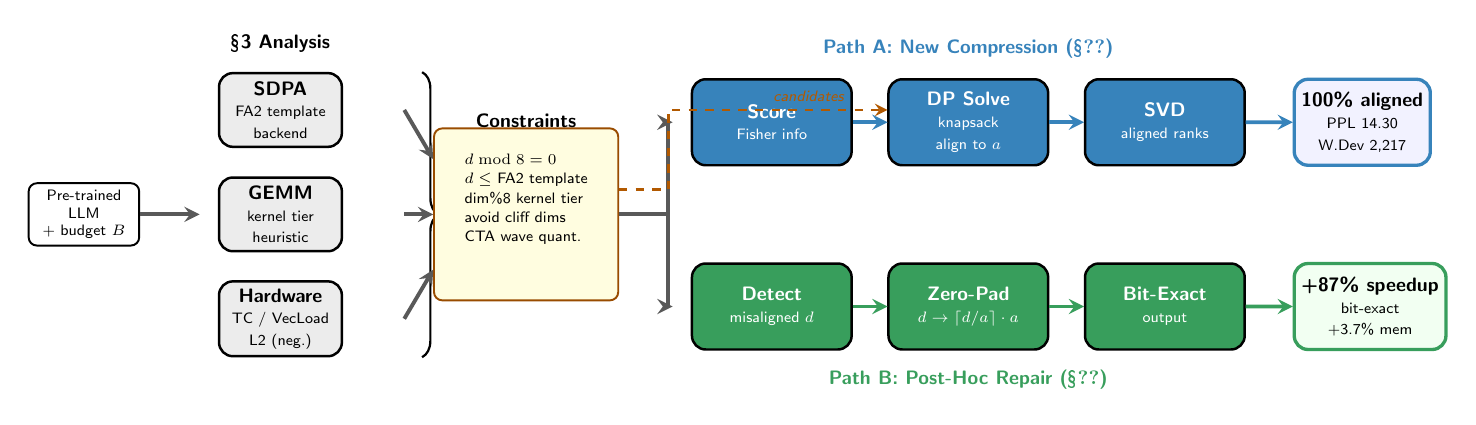
\begin{tikzpicture}[scale=0.78, every node/.style={scale=0.78},
    >=stealth,
    % Colors
    cblue/.style={fill={rgb,255:red,55;green,131;blue,187}},
    cred/.style={fill={rgb,255:red,211;green,63;blue,73}},
    cgreen/.style={fill={rgb,255:red,56;green,158;blue,92}},
    corange/.style={fill={rgb,255:red,230;green,159;blue,0}},
    cgray/.style={fill=gray!15},
    % Box styles
    phase/.style={draw, rounded corners=5pt, minimum width=2.4cm, minimum height=1.6cm,
                  line width=0.9pt, text=white, font=\sffamily\small, align=center},
    constraint/.style={draw, rounded corners=3pt, minimum width=2.0cm, minimum height=0.7cm,
                       line width=0.7pt, font=\sffamily\scriptsize, align=center,
                       fill=yellow!12, draw=orange!60!black},
    result/.style={draw, rounded corners=5pt, minimum width=2.2cm, minimum height=1.6cm,
                   line width=1.2pt, font=\sffamily\small, align=center},
    lbl/.style={font=\sffamily\small, align=center},
    arrow/.style={->, line width=1.4pt, color=gray!70!black},
    dasharrow/.style={->, line width=1.0pt, dashed, color=gray!50},
  ]

  % ===== LEFT: Analysis (§3) =====
  \node[phase, cgray, text=black, minimum width=2.0cm, minimum height=1.2cm]
    (sdpa) at (0, 1.2) {\textbf{SDPA}\\[-1pt]{\scriptsize FA2 template}\\[-1pt]{\scriptsize backend}};
  \node[phase, cgray, text=black, minimum width=2.0cm, minimum height=1.2cm]
    (gemm) at (0, -0.5) {\textbf{GEMM}\\[-1pt]{\scriptsize kernel tier}\\[-1pt]{\scriptsize heuristic}};
  \node[phase, cgray, text=black, minimum width=2.0cm, minimum height=1.2cm]
    (hw) at (0, -2.2) {\textbf{Hardware}\\[-1pt]{\scriptsize TC / VecLoad}\\[-1pt]{\scriptsize L2 (neg.)}};

  % Brace for analysis
  \node[above=0.15cm of sdpa, font=\sffamily\bfseries\small] {\S3 Analysis};
  \draw[decorate, decoration={brace, amplitude=6pt, raise=2pt}, line width=0.8pt]
    ([xshift=1.2cm]sdpa.north east) -- ([xshift=1.2cm]hw.south east);

  % ===== CENTER: Constraints =====
  \node[constraint, minimum width=3.0cm, minimum height=2.8cm]
    (constraints) at (4.0, -0.5) {};
  \node[above=-0.1cm of constraints.north, font=\sffamily\bfseries\small] {Constraints};
  \node[font=\sffamily\scriptsize, align=left, anchor=north] at ([yshift=-0.3cm]constraints.north) {
    $d \bmod 8 = 0$\\[1pt]
    $d \leq$ FA2 template\\[1pt]
    dim\%8 kernel tier\\[1pt]
    avoid cliff dims\\[1pt]
    CTA wave quant.
  };

  % Arrows: analysis → constraints
  \draw[arrow] ([xshift=1.0cm]sdpa.east) -- ([yshift=0.9cm]constraints.west);
  \draw[arrow] ([xshift=1.0cm]gemm.east) -- (constraints.west);
  \draw[arrow] ([xshift=1.0cm]hw.east) -- ([yshift=-0.9cm]constraints.west);

  % ===== RIGHT: Two paths =====
  % Path A: GAC DP (new compression)
  \node[phase, cblue, minimum width=2.6cm, minimum height=1.4cm]
    (score) at (8.0, 1.0) {\textbf{Score}\\[-1pt]{\scriptsize Fisher info}};
  \node[phase, cblue, minimum width=2.6cm, minimum height=1.4cm]
    (dp) at (11.2, 1.0) {\textbf{DP Solve}\\[-1pt]{\scriptsize knapsack}\\[-1pt]{\scriptsize align to $a$}};
  \node[phase, cblue, minimum width=2.6cm, minimum height=1.4cm]
    (svd) at (14.4, 1.0) {\textbf{SVD}\\[-1pt]{\scriptsize aligned ranks}};

  % Path B: Dimension Repair (existing model)
  \node[phase, cgreen, minimum width=2.6cm, minimum height=1.4cm]
    (detect) at (8.0, -2.0) {\textbf{Detect}\\[-1pt]{\scriptsize misaligned $d$}};
  \node[phase, cgreen, minimum width=2.6cm, minimum height=1.4cm]
    (pad) at (11.2, -2.0) {\textbf{Zero-Pad}\\[-1pt]{\scriptsize $d \to \lceil d/a\rceil \cdot a$}};
  \node[phase, cgreen, minimum width=2.6cm, minimum height=1.4cm]
    (exact) at (14.4, -2.0) {\textbf{Bit-Exact}\\[-1pt]{\scriptsize output}};

  % Arrows within paths
  \draw[arrow, color={rgb,255:red,55;green,131;blue,187}] (score) -- (dp);
  \draw[arrow, color={rgb,255:red,55;green,131;blue,187}] (dp) -- (svd);
  \draw[arrow, color={rgb,255:red,56;green,158;blue,92}] (detect) -- (pad);
  \draw[arrow, color={rgb,255:red,56;green,158;blue,92}] (pad) -- (exact);

  % Constraints → paths
  \draw[arrow] (constraints.east) -- ++(0.8,0) |- ([xshift=-0.3cm]score.west)
    node[pos=0.25, above, font=\sffamily\scriptsize\itshape] {};
  \draw[arrow] (constraints.east) -- ++(0.8,0) |- ([xshift=-0.3cm]detect.west);

  % Constraints feeds into DP
  \draw[dasharrow, color=orange!70!black]
    ([yshift=0.4cm]constraints.east) -- ++(0.8,0) |- ([yshift=0.2cm]dp.west)
    node[pos=0.82, above, font=\sffamily\scriptsize\itshape, text=orange!70!black] {candidates};

  % Path labels
  \node[above=0.15cm of dp, font=\sffamily\bfseries\small, text={rgb,255:red,55;green,131;blue,187}]
    {Path A: New Compression (\S\ref{sec:gac})};
  \node[below=0.15cm of pad, font=\sffamily\bfseries\small, text={rgb,255:red,56;green,158;blue,92}]
    {Path B: Post-Hoc Repair (\S\ref{sec:repair})};

  % Results on the right
  \node[result, fill=blue!5, draw={rgb,255:red,55;green,131;blue,187},
        right=0.6cm of svd, minimum height=1.4cm] (resA) {
    {\small\bfseries 100\% aligned}\\[-1pt]
    {\scriptsize PPL 14.30}\\[-1pt]
    {\scriptsize W.Dev 2{,}217}
  };
  \node[result, fill=green!5, draw={rgb,255:red,56;green,158;blue,92},
        right=0.6cm of exact, minimum height=1.4cm] (resB) {
    {\small\bfseries +87\% speedup}\\[-1pt]
    {\scriptsize bit-exact}\\[-1pt]
    {\scriptsize +3.7\% mem}
  };
  \draw[arrow, color={rgb,255:red,55;green,131;blue,187}] (svd) -- (resA);
  \draw[arrow, color={rgb,255:red,56;green,158;blue,92}] (exact) -- (resB);

  % Input on the left
  \node[draw, rounded corners=3pt, fill=white, line width=0.7pt,
        font=\sffamily\scriptsize, align=center, minimum width=1.8cm]
    (input) at (-3.2, -0.5) {Pre-trained\\LLM\\+ budget $B$};
  \draw[arrow] (input) -- ([xshift=-0.3cm]gemm.west |- input);

\end{tikzpicture}
\caption{\textbf{GAC framework overview.}
Analysis (\S\ref{sec:analysis}) extracts alignment constraints from three layers (SDPA, GEMM, hardware).
These constraints drive two complementary solutions:
\emph{Path~A}---alignment-aware rank allocation via multi-choice knapsack DP for new compression;
\emph{Path~B}---zero-padding repair for already-compressed models.
Both paths produce fully-aligned dimensions with no accuracy loss (DP) or bit-exact output preservation (repair).}
\label{fig:gac_framework}
\end{figure*}

\begin{figure*}[t]
\centering
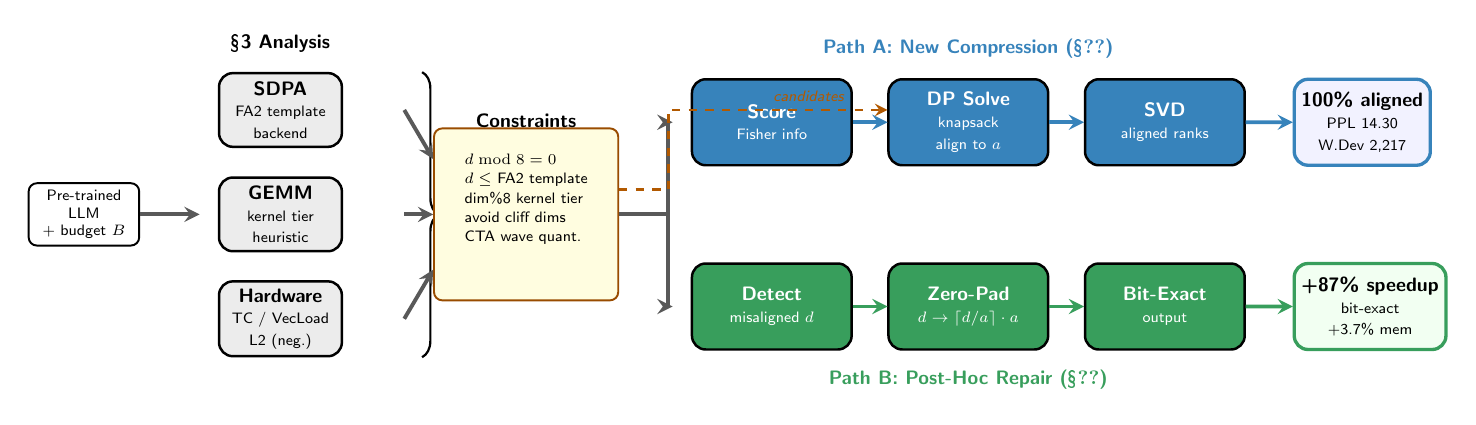
\begin{tikzpicture}[scale=0.78, every node/.style={scale=0.78},
    >=stealth,
    % Colors
    cblue/.style={fill={rgb,255:red,55;green,131;blue,187}},
    cred/.style={fill={rgb,255:red,211;green,63;blue,73}},
    cgreen/.style={fill={rgb,255:red,56;green,158;blue,92}},
    corange/.style={fill={rgb,255:red,230;green,159;blue,0}},
    cgray/.style={fill=gray!15},
    % Box styles
    phase/.style={draw, rounded corners=5pt, minimum width=2.4cm, minimum height=1.6cm,
                  line width=0.9pt, text=white, font=\sffamily\small, align=center},
    constraint/.style={draw, rounded corners=3pt, minimum width=2.0cm, minimum height=0.7cm,
                       line width=0.7pt, font=\sffamily\scriptsize, align=center,
                       fill=yellow!12, draw=orange!60!black},
    result/.style={draw, rounded corners=5pt, minimum width=2.2cm, minimum height=1.6cm,
                   line width=1.2pt, font=\sffamily\small, align=center},
    lbl/.style={font=\sffamily\small, align=center},
    arrow/.style={->, line width=1.4pt, color=gray!70!black},
    dasharrow/.style={->, line width=1.0pt, dashed, color=gray!50},
  ]

  % ===== LEFT: Analysis (§3) =====
  \node[phase, cgray, text=black, minimum width=2.0cm, minimum height=1.2cm]
    (sdpa) at (0, 1.2) {\textbf{SDPA}\\[-1pt]{\scriptsize FA2 template}\\[-1pt]{\scriptsize backend}};
  \node[phase, cgray, text=black, minimum width=2.0cm, minimum height=1.2cm]
    (gemm) at (0, -0.5) {\textbf{GEMM}\\[-1pt]{\scriptsize kernel tier}\\[-1pt]{\scriptsize heuristic}};
  \node[phase, cgray, text=black, minimum width=2.0cm, minimum height=1.2cm]
    (hw) at (0, -2.2) {\textbf{Hardware}\\[-1pt]{\scriptsize TC / VecLoad}\\[-1pt]{\scriptsize L2 (neg.)}};

  % Brace for analysis
  \node[above=0.15cm of sdpa, font=\sffamily\bfseries\small] {\S3 Analysis};
  \draw[decorate, decoration={brace, amplitude=6pt, raise=2pt}, line width=0.8pt]
    ([xshift=1.2cm]sdpa.north east) -- ([xshift=1.2cm]hw.south east);

  % ===== CENTER: Constraints =====
  \node[constraint, minimum width=3.0cm, minimum height=2.8cm]
    (constraints) at (4.0, -0.5) {};
  \node[above=-0.1cm of constraints.north, font=\sffamily\bfseries\small] {Constraints};
  \node[font=\sffamily\scriptsize, align=left, anchor=north] at ([yshift=-0.3cm]constraints.north) {
    $d \bmod 8 = 0$\\[1pt]
    $d \leq$ FA2 template\\[1pt]
    dim\%8 kernel tier\\[1pt]
    avoid cliff dims\\[1pt]
    CTA wave quant.
  };

  % Arrows: analysis → constraints
  \draw[arrow] ([xshift=1.0cm]sdpa.east) -- ([yshift=0.9cm]constraints.west);
  \draw[arrow] ([xshift=1.0cm]gemm.east) -- (constraints.west);
  \draw[arrow] ([xshift=1.0cm]hw.east) -- ([yshift=-0.9cm]constraints.west);

  % ===== RIGHT: Two paths =====
  % Path A: GAC DP (new compression)
  \node[phase, cblue, minimum width=2.6cm, minimum height=1.4cm]
    (score) at (8.0, 1.0) {\textbf{Score}\\[-1pt]{\scriptsize Fisher info}};
  \node[phase, cblue, minimum width=2.6cm, minimum height=1.4cm]
    (dp) at (11.2, 1.0) {\textbf{DP Solve}\\[-1pt]{\scriptsize knapsack}\\[-1pt]{\scriptsize align to $a$}};
  \node[phase, cblue, minimum width=2.6cm, minimum height=1.4cm]
    (svd) at (14.4, 1.0) {\textbf{SVD}\\[-1pt]{\scriptsize aligned ranks}};

  % Path B: Dimension Repair (existing model)
  \node[phase, cgreen, minimum width=2.6cm, minimum height=1.4cm]
    (detect) at (8.0, -2.0) {\textbf{Detect}\\[-1pt]{\scriptsize misaligned $d$}};
  \node[phase, cgreen, minimum width=2.6cm, minimum height=1.4cm]
    (pad) at (11.2, -2.0) {\textbf{Zero-Pad}\\[-1pt]{\scriptsize $d \to \lceil d/a\rceil \cdot a$}};
  \node[phase, cgreen, minimum width=2.6cm, minimum height=1.4cm]
    (exact) at (14.4, -2.0) {\textbf{Bit-Exact}\\[-1pt]{\scriptsize output}};

  % Arrows within paths
  \draw[arrow, color={rgb,255:red,55;green,131;blue,187}] (score) -- (dp);
  \draw[arrow, color={rgb,255:red,55;green,131;blue,187}] (dp) -- (svd);
  \draw[arrow, color={rgb,255:red,56;green,158;blue,92}] (detect) -- (pad);
  \draw[arrow, color={rgb,255:red,56;green,158;blue,92}] (pad) -- (exact);

  % Constraints → paths
  \draw[arrow] (constraints.east) -- ++(0.8,0) |- ([xshift=-0.3cm]score.west)
    node[pos=0.25, above, font=\sffamily\scriptsize\itshape] {};
  \draw[arrow] (constraints.east) -- ++(0.8,0) |- ([xshift=-0.3cm]detect.west);

  % Constraints feeds into DP
  \draw[dasharrow, color=orange!70!black]
    ([yshift=0.4cm]constraints.east) -- ++(0.8,0) |- ([yshift=0.2cm]dp.west)
    node[pos=0.82, above, font=\sffamily\scriptsize\itshape, text=orange!70!black] {candidates};

  % Path labels
  \node[above=0.15cm of dp, font=\sffamily\bfseries\small, text={rgb,255:red,55;green,131;blue,187}]
    {Path A: New Compression (\S\ref{sec:gac})};
  \node[below=0.15cm of pad, font=\sffamily\bfseries\small, text={rgb,255:red,56;green,158;blue,92}]
    {Path B: Post-Hoc Repair (\S\ref{sec:repair})};

  % Results on the right
  \node[result, fill=blue!5, draw={rgb,255:red,55;green,131;blue,187},
        right=0.6cm of svd, minimum height=1.4cm] (resA) {
    {\small\bfseries 100\% aligned}\\[-1pt]
    {\scriptsize PPL 14.30}\\[-1pt]
    {\scriptsize W.Dev 2{,}217}
  };
  \node[result, fill=green!5, draw={rgb,255:red,56;green,158;blue,92},
        right=0.6cm of exact, minimum height=1.4cm] (resB) {
    {\small\bfseries +87\% speedup}\\[-1pt]
    {\scriptsize bit-exact}\\[-1pt]
    {\scriptsize +3.7\% mem}
  };
  \draw[arrow, color={rgb,255:red,55;green,131;blue,187}] (svd) -- (resA);
  \draw[arrow, color={rgb,255:red,56;green,158;blue,92}] (exact) -- (resB);

  % Input on the left
  \node[draw, rounded corners=3pt, fill=white, line width=0.7pt,
        font=\sffamily\scriptsize, align=center, minimum width=1.8cm]
    (input) at (-3.2, -0.5) {Pre-trained\\LLM\\+ budget $B$};
  \draw[arrow] (input) -- ([xshift=-0.3cm]gemm.west |- input);

\end{tikzpicture}
\caption{\textbf{GAC framework overview.}
Analysis (\S\ref{sec:analysis}) extracts alignment constraints from three layers (SDPA, GEMM, hardware).
These constraints drive two complementary solutions:
\emph{Path~A}---alignment-aware rank allocation via multi-choice knapsack DP for new compression;
\emph{Path~B}---zero-padding repair for already-compressed models.
Both paths produce fully-aligned dimensions with no accuracy loss (DP) or bit-exact output preservation (repair).}
\label{fig:gac_framework}
\end{figure*}

\begin{figure*}[t]
\centering
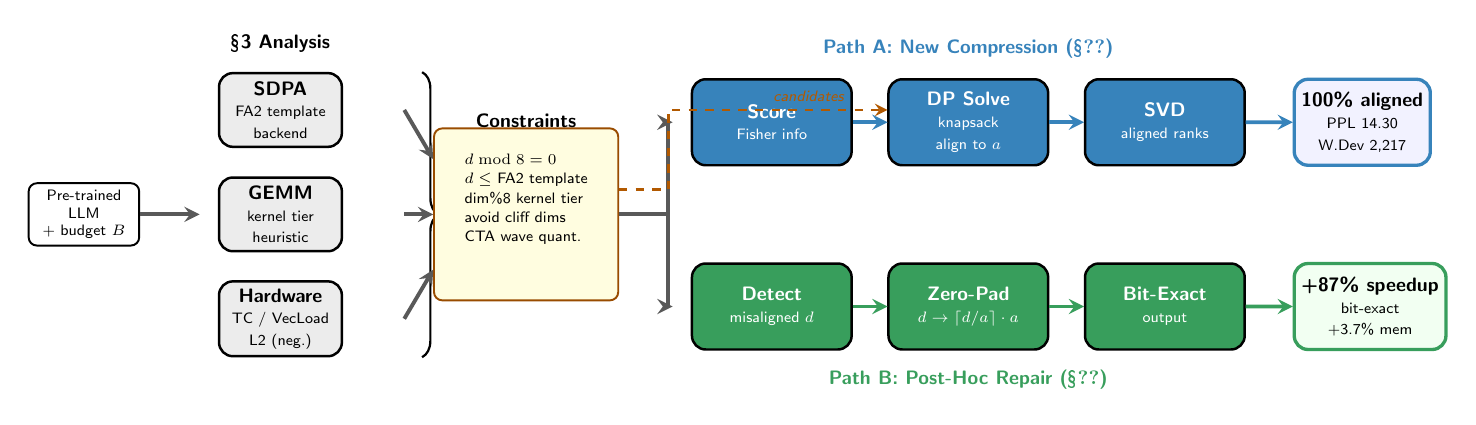
\begin{tikzpicture}[scale=0.78, every node/.style={scale=0.78},
    >=stealth,
    % Colors
    cblue/.style={fill={rgb,255:red,55;green,131;blue,187}},
    cred/.style={fill={rgb,255:red,211;green,63;blue,73}},
    cgreen/.style={fill={rgb,255:red,56;green,158;blue,92}},
    corange/.style={fill={rgb,255:red,230;green,159;blue,0}},
    cgray/.style={fill=gray!15},
    % Box styles
    phase/.style={draw, rounded corners=5pt, minimum width=2.4cm, minimum height=1.6cm,
                  line width=0.9pt, text=white, font=\sffamily\small, align=center},
    constraint/.style={draw, rounded corners=3pt, minimum width=2.0cm, minimum height=0.7cm,
                       line width=0.7pt, font=\sffamily\scriptsize, align=center,
                       fill=yellow!12, draw=orange!60!black},
    result/.style={draw, rounded corners=5pt, minimum width=2.2cm, minimum height=1.6cm,
                   line width=1.2pt, font=\sffamily\small, align=center},
    lbl/.style={font=\sffamily\small, align=center},
    arrow/.style={->, line width=1.4pt, color=gray!70!black},
    dasharrow/.style={->, line width=1.0pt, dashed, color=gray!50},
  ]

  % ===== LEFT: Analysis (§3) =====
  \node[phase, cgray, text=black, minimum width=2.0cm, minimum height=1.2cm]
    (sdpa) at (0, 1.2) {\textbf{SDPA}\\[-1pt]{\scriptsize FA2 template}\\[-1pt]{\scriptsize backend}};
  \node[phase, cgray, text=black, minimum width=2.0cm, minimum height=1.2cm]
    (gemm) at (0, -0.5) {\textbf{GEMM}\\[-1pt]{\scriptsize kernel tier}\\[-1pt]{\scriptsize heuristic}};
  \node[phase, cgray, text=black, minimum width=2.0cm, minimum height=1.2cm]
    (hw) at (0, -2.2) {\textbf{Hardware}\\[-1pt]{\scriptsize TC / VecLoad}\\[-1pt]{\scriptsize L2 (neg.)}};

  % Brace for analysis
  \node[above=0.15cm of sdpa, font=\sffamily\bfseries\small] {\S3 Analysis};
  \draw[decorate, decoration={brace, amplitude=6pt, raise=2pt}, line width=0.8pt]
    ([xshift=1.2cm]sdpa.north east) -- ([xshift=1.2cm]hw.south east);

  % ===== CENTER: Constraints =====
  \node[constraint, minimum width=3.0cm, minimum height=2.8cm]
    (constraints) at (4.0, -0.5) {};
  \node[above=-0.1cm of constraints.north, font=\sffamily\bfseries\small] {Constraints};
  \node[font=\sffamily\scriptsize, align=left, anchor=north] at ([yshift=-0.3cm]constraints.north) {
    $d \bmod 8 = 0$\\[1pt]
    $d \leq$ FA2 template\\[1pt]
    dim\%8 kernel tier\\[1pt]
    avoid cliff dims\\[1pt]
    CTA wave quant.
  };

  % Arrows: analysis → constraints
  \draw[arrow] ([xshift=1.0cm]sdpa.east) -- ([yshift=0.9cm]constraints.west);
  \draw[arrow] ([xshift=1.0cm]gemm.east) -- (constraints.west);
  \draw[arrow] ([xshift=1.0cm]hw.east) -- ([yshift=-0.9cm]constraints.west);

  % ===== RIGHT: Two paths =====
  % Path A: GAC DP (new compression)
  \node[phase, cblue, minimum width=2.6cm, minimum height=1.4cm]
    (score) at (8.0, 1.0) {\textbf{Score}\\[-1pt]{\scriptsize Fisher info}};
  \node[phase, cblue, minimum width=2.6cm, minimum height=1.4cm]
    (dp) at (11.2, 1.0) {\textbf{DP Solve}\\[-1pt]{\scriptsize knapsack}\\[-1pt]{\scriptsize align to $a$}};
  \node[phase, cblue, minimum width=2.6cm, minimum height=1.4cm]
    (svd) at (14.4, 1.0) {\textbf{SVD}\\[-1pt]{\scriptsize aligned ranks}};

  % Path B: Dimension Repair (existing model)
  \node[phase, cgreen, minimum width=2.6cm, minimum height=1.4cm]
    (detect) at (8.0, -2.0) {\textbf{Detect}\\[-1pt]{\scriptsize misaligned $d$}};
  \node[phase, cgreen, minimum width=2.6cm, minimum height=1.4cm]
    (pad) at (11.2, -2.0) {\textbf{Zero-Pad}\\[-1pt]{\scriptsize $d \to \lceil d/a\rceil \cdot a$}};
  \node[phase, cgreen, minimum width=2.6cm, minimum height=1.4cm]
    (exact) at (14.4, -2.0) {\textbf{Bit-Exact}\\[-1pt]{\scriptsize output}};

  % Arrows within paths
  \draw[arrow, color={rgb,255:red,55;green,131;blue,187}] (score) -- (dp);
  \draw[arrow, color={rgb,255:red,55;green,131;blue,187}] (dp) -- (svd);
  \draw[arrow, color={rgb,255:red,56;green,158;blue,92}] (detect) -- (pad);
  \draw[arrow, color={rgb,255:red,56;green,158;blue,92}] (pad) -- (exact);

  % Constraints → paths
  \draw[arrow] (constraints.east) -- ++(0.8,0) |- ([xshift=-0.3cm]score.west)
    node[pos=0.25, above, font=\sffamily\scriptsize\itshape] {};
  \draw[arrow] (constraints.east) -- ++(0.8,0) |- ([xshift=-0.3cm]detect.west);

  % Constraints feeds into DP
  \draw[dasharrow, color=orange!70!black]
    ([yshift=0.4cm]constraints.east) -- ++(0.8,0) |- ([yshift=0.2cm]dp.west)
    node[pos=0.82, above, font=\sffamily\scriptsize\itshape, text=orange!70!black] {candidates};

  % Path labels
  \node[above=0.15cm of dp, font=\sffamily\bfseries\small, text={rgb,255:red,55;green,131;blue,187}]
    {Path A: New Compression (\S\ref{sec:gac})};
  \node[below=0.15cm of pad, font=\sffamily\bfseries\small, text={rgb,255:red,56;green,158;blue,92}]
    {Path B: Post-Hoc Repair (\S\ref{sec:repair})};

  % Results on the right
  \node[result, fill=blue!5, draw={rgb,255:red,55;green,131;blue,187},
        right=0.6cm of svd, minimum height=1.4cm] (resA) {
    {\small\bfseries 100\% aligned}\\[-1pt]
    {\scriptsize PPL 14.30}\\[-1pt]
    {\scriptsize W.Dev 2{,}217}
  };
  \node[result, fill=green!5, draw={rgb,255:red,56;green,158;blue,92},
        right=0.6cm of exact, minimum height=1.4cm] (resB) {
    {\small\bfseries +87\% speedup}\\[-1pt]
    {\scriptsize bit-exact}\\[-1pt]
    {\scriptsize +3.7\% mem}
  };
  \draw[arrow, color={rgb,255:red,55;green,131;blue,187}] (svd) -- (resA);
  \draw[arrow, color={rgb,255:red,56;green,158;blue,92}] (exact) -- (resB);

  % Input on the left
  \node[draw, rounded corners=3pt, fill=white, line width=0.7pt,
        font=\sffamily\scriptsize, align=center, minimum width=1.8cm]
    (input) at (-3.2, -0.5) {Pre-trained\\LLM\\+ budget $B$};
  \draw[arrow] (input) -- ([xshift=-0.3cm]gemm.west |- input);

\end{tikzpicture}
\caption{\textbf{GAC framework overview.}
Analysis (\S\ref{sec:analysis}) extracts alignment constraints from three layers (SDPA, GEMM, hardware).
These constraints drive two complementary solutions:
\emph{Path~A}---alignment-aware rank allocation via multi-choice knapsack DP for new compression;
\emph{Path~B}---zero-padding repair for already-compressed models.
Both paths produce fully-aligned dimensions with no accuracy loss (DP) or bit-exact output preservation (repair).}
\label{fig:gac_framework}
\end{figure*}


\subsection{Problem Formulation}

Given a compression budget $B$ (total rank across all projections), layer sensitivities $\{s_i\}$ (e.g., Fisher information), and alignment constraint $a$ (default 8), we seek rank allocations $\{r_i\}$ that minimize accuracy degradation while maintaining hardware alignment:
\begin{equation}
\min_{\{r_i\}} \sum_{i=1}^{n} s_i \cdot |r_i - r_i^*| \;\;\text{s.t.}\;\; \sum_{i} r_i \cdot g = B,\; r_i \bmod a = 0 \;\forall i
\label{eq:gac}
\end{equation}
where $r_i^*$ is the ideal (unconstrained, Fisher-proportional) rank for projection $i$, $g$ is the number of groups per projection, and the objective is a sensitivity-weighted deviation proxy for accuracy loss.

\subsection{Multi-Choice Knapsack DP}

We solve Eq.~\ref{eq:gac} via dynamic programming.
For each of $n$ projections, we generate candidate ranks: multiples of $a$ near $r_i^*$ (search radius $\pm 8a$), with costs $c_{ij} = s_i \cdot |r_{ij} - r_i^*|$ and weights $w_{ij} = r_{ij} \cdot g$.
The DP table $D[i][b]$ stores the minimum cost using projections $1..i$ with total weight $b$:
\[
D[i][b] = \min_{j} \left\{ D[i{-}1][b - w_{ij}] + c_{ij} \right\}
\]
Complexity: $O(n \cdot B/a \cdot |C|)$ where $|C| \approx 17$ candidates per projection.
For Llama-3-8B ($n$=64, $B$=46080), this solves in $<$2s on CPU.

\paragraph{Key Insight.}
Unlike naive round-to-nearest (independent per projection), GAC DP performs \emph{global} optimization: sensitive layers round \emph{up} to preserve accuracy while insensitive layers round \emph{down} to stay within budget.
This achieves lower weighted deviation (better accuracy proxy) than any independent rounding strategy.

\paragraph{Candidate Generation.}
For each projection $i$ with ideal rank $r_i^*$, we generate candidates:
\[
C_i = \{r : r = ka,\; |r - r_i^*| \leq 8a,\; a \leq r \leq d_{\max}\}
\]
This produces $|C_i| \approx 17$ candidates per projection.
Cliff dimensions (from profiling) can be excluded from $C_i$, preventing kernel heuristic traps.

\paragraph{Algorithm.}
The procedure is:
\begin{enumerate}
  \setlength\itemsep{1pt}
\item \textbf{Score}: Compute per-projection sensitivity $s_i$ via Fisher information (or other importance metric) on calibration data.
\item \textbf{Allocate}: Distribute total budget $B$ proportionally to $s_i$; cap at $d_{\max}$ and iteratively redistribute surplus from capped projections.
\item \textbf{Solve DP}: For each projection, generate aligned candidates $C_i$. Run multi-choice knapsack DP with budget $B/(a \cdot g)$ units. Backtrack to recover optimal aligned ranks.
\item \textbf{Decompose}: Apply SVD with the selected aligned ranks. No post-hoc padding needed.
\end{enumerate}
Steps 1--3 run on CPU in $<$2 seconds for 64 projections.

\subsection{Dimension Repair (Post-Hoc)}
\label{sec:repair}

For already-compressed models where re-decomposition is impractical, we pad misaligned dimensions to the nearest $a$-multiple: $d_{\text{pad}} = \lceil d/a \rceil \times a$.
Zero-padding preserves outputs exactly ($y' = [Wx{+}b;\,\mathbf{0}]$), making it \textbf{bit-exact}---no retraining required.
Two strategies: MINIMAL ($a$=8, 3.7\% overhead) and OPTIMAL ($a$=16, 7.2\% overhead).


%% ===========================================
%% 5. EVALUATION
%% ===========================================
\section{Evaluation}
\label{sec:eval}

\subsection{Rank Allocation Comparison}
\label{sec:rank_comparison}

We compare five allocation strategies:

\begin{itemize}
  \setlength\itemsep{0pt}
\item \textbf{Baseline}: Uncompressed Llama-3-8B (8.03B).
\item \textbf{PaLU actual}: Production PaLU checkpoint with finetuning~\cite{palu}.
\item \textbf{GAC DP}: Our multi-choice knapsack (align to 8).
\item \textbf{Round-to-8}: Independent rounding, sensitivity fill.
\item \textbf{Unaligned}: Floor to nearest integer (no alignment).
\end{itemize}

Table~\ref{tab:gac} shows the results.
All compressed variants use identical total parameters (7.97B) and rank budget.
Perplexity is measured on WikiText-2 (252K tokens, block size 512).

\begin{table}[t]
\centering
\caption{\textbf{Main result}: Rank allocation comparison on Llama-3-8B ($r$=0.7). All compressed strategies use the same total rank budget (46,080). \emph{W.Dev}: sensitivity-weighted deviation from ideal ranks (lower = better). \emph{Lat.}: estimated GEMM latency penalty.}
\label{tab:gac}
\small
\setlength{\tabcolsep}{3.5pt}
\begin{tabular}{@{}lrrrrr@{}}
\toprule
Strategy & PPL$\downarrow$ & Aligned & W.Dev$\downarrow$ & Lat. \\
\midrule
Baseline (full) & 11.35 & --- & --- & 1.00$\times$ \\
PaLU (finetuned)  & 12.91 & 64/64 & 11{,}711 & 1.00$\times$ \\
\midrule
\textbf{GAC DP} & \textbf{14.30} & \textbf{64/64} & \textbf{2{,}217} & \textbf{1.00$\times$} \\
Round-to-8 & 14.37 & 64/64 & 2{,}841 & 1.00$\times$ \\
Unaligned & 14.44 & 38/64 & 2{,}723 & 1.10$\times$ \\
\bottomrule
\end{tabular}
\end{table}

\paragraph{GAC DP achieves Pareto dominance.}
Among SVD-only methods (no finetuning), GAC DP has the best perplexity (14.30 vs 14.37, 14.44), the lowest weighted deviation (2,217 vs 2,841), and 100\% alignment.
The unaligned strategy suffers a double penalty: worst perplexity \emph{and} 10\% latency overhead from 26 misaligned projections.

\paragraph{PaLU gap analysis.}
PaLU's superior perplexity (12.91) comes from post-compression finetuning, not allocation quality---its weighted deviation (11,711) is 5$\times$ worse than GAC DP, indicating near-uniform allocation that ignores per-layer sensitivity.

\subsection{Per-Layer Rank Distribution}

Figure~\ref{fig:gac_ranks} visualizes per-layer ranks across strategies.
GAC DP (blue) tracks the ideal Fisher-proportional allocation while maintaining 8-alignment; it allocates more rank to sensitive layers (14, 27--31) and less to insensitive ones, achieving global optimality under the budget constraint.
The unaligned strategy follows the ideal closely but produces irregular values (117, 149, 305) that trigger Tier 2/3 kernels.

\begin{figure}[t]
\centering
\includegraphics[width=\columnwidth]{figures/fig_gac_ranks.pdf}
\caption{Per-layer rank allocation for $W_K$ and $W_V$ projections. GAC DP (blue) maintains alignment while tracking ideal (gray dotted). Unaligned (red) produces non-8-aligned ranks.}
\label{fig:gac_ranks}
\end{figure}

\subsection{Applicability: When Does Alignment Matter?}
\label{sec:applicability}

The performance impact depends on whether misaligned dimensions reach performance-critical operations.

\paragraph{Negative: projection-based SVD.}
In RAP~SVD, layers $W_A$ (hidden$\to$latent) and $W_B$ (latent$\to$head\_dim) restore aligned head\_dim\,=\,128 \emph{before} SDPA, so repair provides no benefit.
Table~\ref{tab:rap_e2e} confirms: --0.8\% prefill, --0.9\% decode (Llama-3-8B, $r{=}0.8$, $d{=}102{\to}104$).
This negative result validates that our framework correctly identifies when \emph{not} to apply repair.

\begin{table}[h]
\centering
\caption{RAP SVD E2E ($d$=102$\to$104). No speedup: SDPA operates on aligned head\_dim=128.}
\label{tab:rap_e2e}
\small
\begin{tabular}{lrrr}
\toprule
Phase & Misaligned & Repaired & $\Delta$ \\
\midrule
Prefill (ms) & 290.5 & 292.9 & --0.8\% \\
Decode (tok/s) & 1009 & 1000 & --0.9\% \\
Memory (MB) & 15451 & 15461 & +0.1\% \\
\bottomrule
\end{tabular}
\end{table}

\paragraph{Positive: Direct compression.}
When compressed dimensions flow directly to SDPA, repair achieves substantial speedups.
Table~\ref{tab:direct_sdpa_main} shows per-dimension results across 45 workloads ($B{\in}\{1,4,8\}$, $S{\in}\{512,1024,2048\}$): mean 86.9\% speedup, with higher gains at larger batch sizes.

\begin{table}[t]
\centering
\caption{SDPA speedup for direct compression scenario (45 workloads).}
\label{tab:direct_sdpa_main}
\small
\begin{tabular}{llrrrr}
\toprule
Misaligned & Repaired & Avg & Std & Min & Max \\
\midrule
107 & 112 & \textbf{78.5\%} & 29.2\% & 46.3\% & 139.5\% \\
114 & 120 & \textbf{80.2\%} & 29.0\% & 46.9\% & 139.4\% \\
117 & 120 & \textbf{80.7\%} & 28.8\% & 47.0\% & 139.5\% \\
121 & 128 & \textbf{97.0\%} & 38.4\% & 55.1\% & 177.2\% \\
125 & 128 & \textbf{98.1\%} & 39.7\% & 55.4\% & 181.4\% \\
\midrule
\multicolumn{2}{l}{\textbf{Overall}} & \textbf{86.9\%} & 34.5\% & 46.3\% & 181.4\% \\
\bottomrule
\end{tabular}
\end{table}

\begin{table}[t]
\centering
\setlength{\tabcolsep}{4pt}
\caption{Applicability framework (validated by experiments).}
\label{tab:applicability}
\small
\begin{tabular}{@{}p{2.4cm}p{1.6cm}ll@{}}
\toprule
\textbf{Architecture} & \textbf{SDPA dim} & \textbf{Effect} & \textbf{Val.} \\
\midrule
\textbf{Direct SVD} & Misaligned & \textbf{+86.9\%} & \S\ref{sec:applicability} \\
\textbf{Projection} (RAP) & Aligned & --0.8\% & \S\ref{sec:applicability} \\
\textbf{Quantization} & Unchanged & N/A & --- \\
\bottomrule
\end{tabular}
\end{table}

\paragraph{Kernel-level validation.}
GEMM with $K{=}107$ takes 0.089\,ms vs $K{=}112$ at 0.050\,ms (44\% improvement).
SDPA repair ($d{=}107{\to}112$) achieves 27.8\% speedup with 4.7\% overhead (Appendix~\ref{app:repair}).
MINIMAL strategy averages 22\% speedup, 3.7\% overhead.

\subsection{End-to-End Inference Performance}

To put dimensional collapse in context, we measure end-to-end inference performance of aligned PaLU compression on Llama-3-8B ($B$=4, $S$=2048, A100 80GB).
PaLU (which enforces 32-alignment, avoiding dimensional collapse) achieves:
\textbf{Prefill}: 9,672 tok/s (--2.0\% vs baseline 9,870 tok/s, due to extra projection layers).
\textbf{Decode}: 1,371 tok/s (\textbf{11.5$\times$} vs baseline 119 tok/s, due to KV cache compression).
The decode speedup demonstrates the value of compression when alignment is maintained.
Without alignment (using unconstrained ranks), the 10.4\% GEMM latency penalty from Table~\ref{tab:gac} would partially offset these gains---GAC ensures the full speedup is realized.

\subsection{Accuracy Preservation}

Zero-padding guarantees \textbf{bit-exact output preservation}: $y'[0{:}d_{out}] = y$.
For attention, zero-valued dimensions contribute nothing to softmax scores, making padding semantically neutral.
Unit tests confirm identical outputs (30/30 passed).
WikiText-2 perplexity on RAP SVD ($r$=0.8, $d$=102): baseline 11.08, repaired 92.39 (identical to unrepaired---higher PPL from compression, not repair).

\subsection{Discussion}

GAC operates at \emph{compression time}, selecting aligned ranks before decomposition---no memory overhead, no approximation.
Dimension repair operates \emph{post-hoc} via zero-padding.
These are complementary: GAC is preferred for new pipelines; repair handles legacy models.

The perplexity ordering (GAC DP $<$ Round-to-8 $<$ Unaligned) at the same budget demonstrates that alignment constraints \emph{improve} accuracy when combined with global optimization.
Naive rounding distorts the sensitivity-proportional allocation; GAC DP restores it while respecting hardware constraints.

The PPL gap between finetuned PaLU (12.91) and SVD-only GAC (14.30) comes from post-compression finetuning---not allocation strategy.
Applying finetuning \emph{after} GAC allocation should close this gap while retaining alignment benefits.

\paragraph{Practical implications.}
For compression framework developers: GAC adds $<$2s of CPU computation to the rank selection step (negligible vs hours of SVD decomposition and finetuning).
For serving system developers: GAC eliminates the need for runtime padding (TensorRT) or dimension rejection (vLLM) by ensuring all dimensions are GPU-friendly at compile time.
The alignment constraint is not merely a performance optimization but a correctness requirement for some backends (MEM\_EFFICIENT SDPA rejects non-8-aligned dimensions entirely).


%% ===========================================
%% 6. RELATED WORK
%% ===========================================
\section{Related Work}
\label{sec:related}

\paragraph{GPU Alignment.}
Tensor Core alignment requirements tighten across generations~\cite{nvidia_tensor_core_evolution2024}: Volta requires $K \bmod 8$, Ampere $K \bmod 16$~\cite{ampere_whitepaper}, Hopper introduces TMA with 128-byte transfers~\cite{nvidia_hopper_whitepaper}.
FlashAttention-3~\cite{flashattention3} \emph{removes} support for head\_dim 96 and 112 on Hopper.
CUTLASS~\cite{cutlass,cutlass_alignment2024} requires 128-bit vectorized accesses.

\paragraph{LLM Compression.}
SVD methods~\cite{palu,svdllm2024,fwsvd2022,gfwsvd2025} can produce irregular ranks; GF-WSVD~\cite{gfwsvd2025} uses Kronecker-factored Fisher for scalable importance scoring but does not constrain output dimensions.
Quantization (GPTQ~\cite{gptq}, AWQ~\cite{awq}) preserves dimensions via fixed-width groups---naturally avoiding dimensional collapse.
KV cache compression~\cite{h2o,quest,pyramidkv} modifies sequence-length dimensions ($M$), which we show is less alignment-sensitive but vulnerable to kernel-switching cliffs.

\paragraph{Hardware-Aware Optimization.}
AMC~\cite{amc2018} pioneered RL-based compression with latency constraints.
HALP~\cite{halp2021} formulates pruning as latency-budgeted optimization.
HALOC~\cite{haloc2023} uses differentiable latency for rank selection.
HAPE~\cite{hape2025} integrates on-device profiling.
\textbf{None explicitly model alignment constraints} as first-class objectives---they measure aggregate latency without isolating dimensional misalignment.
GAC encodes alignment as hard constraints in the knapsack formulation.

\paragraph{Why Prior Work Missed Alignment.}
PaLU enforces 32-multiple alignment (verified across 24 checkpoints) but does not explain why---likely discovered through iterative profiling.
SVD methods~\cite{svdllm2024,fwsvd2022} optimize reconstruction error without hardware constraints---producing 43--91\% misaligned dimensions when unconstrained (\S\ref{sec:analysis}).
Serving systems handle misalignment reactively: FlashAttention-2 adds 30--45\% overhead for non-optimal dimensions; vLLM rejects unsupported head\_dim entirely; TensorRT applies runtime padding.
GAC prevents misalignment at compression time.


%% ===========================================
%% 7. CONCLUSION
%% ===========================================
\section{Conclusion}
\label{sec:conclusion}

We present the first systematic study of dimensional collapse in compressed LLMs, diagnosing how irregular tensor dimensions degrade GPU performance across GEMM (up to 30\%) and SDPA (up to 88\%).
Our GAC framework integrates alignment as a first-class constraint via multi-choice knapsack DP, achieving Pareto dominance: better accuracy (PPL 14.30 vs 14.44) with 100\% alignment at the same parameter budget.

\paragraph{Future Work.}
Finetuning after GAC allocation to close the gap with PaLU (12.91 vs 14.30).
Extension to H100/Blackwell with stricter TMA and FP4/FP8 constraints.
Comprehensive downstream evaluation beyond perplexity.

\paragraph{Limitations.}
All experiments target A100 with Flash\-Attention~2.7.4; GAC currently targets SVD compression.
Extending to pruning and token eviction requires different candidate generation.

\paragraph{Reproducibility.}
Code, scripts, and raw data: \url{https://github.com/[ANONYMIZED]}.

%% ===========================================
%% REFERENCES
%% ===========================================
\clearpage
\bibliographystyle{ACM-Reference-Format}
\bibliography{references}

%% ===========================================
%% APPENDIX
%% ===========================================
\appendix

\section{Dimension Distribution Across Models}
\label{app:scatter}

Figure~\ref{fig:dim_scatter} shows per-layer head dimensions for Llama-3-8B ($r$=0.8) under four importance criteria.
Across all method$\times$projection combinations, 43--91\% of dimensions are not 8-aligned (avg 70.5\%).

\begin{figure*}[h]
\centering
\includegraphics[width=0.9\textwidth]{figures/fig_scatter_llama_r08.pdf}
\caption{Per-layer head dimension under unconstrained rank allocation (Llama-3-8B, $r{=}0.8$).
Green = 8-aligned; red = misaligned. Average 70.5\% misaligned.}
\label{fig:dim_scatter}
\end{figure*}

Figures~\ref{fig:scatter_llama_ratios}--\ref{fig:scatter_mistral_ratios} extend to other retain ratios and Mistral-7B.

\begin{figure*}[h]
\centering
\begin{minipage}{\textwidth}
  \centering
  \includegraphics[width=\textwidth]{figures/fig_scatter_llama_r05.pdf}\\[2pt]
  \includegraphics[width=\textwidth]{figures/fig_scatter_llama_r06.pdf}\\[2pt]
  \includegraphics[width=\textwidth]{figures/fig_scatter_llama_r07.pdf}\\[2pt]
  \includegraphics[width=\textwidth]{figures/fig_scatter_llama_r09.pdf}
\end{minipage}
\caption{Llama-3-8B dimension distributions at retain ratios 0.5, 0.6, 0.7, 0.9.}
\label{fig:scatter_llama_ratios}
\end{figure*}

\begin{figure*}[h]
\centering
\begin{minipage}{\textwidth}
  \centering
  \includegraphics[width=\textwidth]{figures/fig_scatter_mistral_r05.pdf}\\[2pt]
  \includegraphics[width=\textwidth]{figures/fig_scatter_mistral_r06.pdf}\\[2pt]
  \includegraphics[width=\textwidth]{figures/fig_scatter_mistral_r07.pdf}\\[2pt]
  \includegraphics[width=\textwidth]{figures/fig_scatter_mistral_r08.pdf}\\[2pt]
  \includegraphics[width=\textwidth]{figures/fig_scatter_mistral_r09.pdf}
\end{minipage}
\caption{Mistral-7B dimension distributions at retain ratios 0.5--0.9.}
\label{fig:scatter_mistral_ratios}
\end{figure*}

\section{SDPA Repair Details}
\label{app:repair}

\begin{table}[h]
\centering
\caption{SDPA repair latency (ms, $B$=4, $S$=2048, $H$=32).}
\label{tab:repair_detail}
\small
\begin{tabular}{lrrrrr}
\toprule
$d$ & Orig & Min & Opt & $\Delta$Min & $\Delta$Opt \\
\midrule
107 & 2.06 & 1.49 & 1.51 & \textbf{+27.8\%} & +27.0\% \\
114 & 2.05 & 1.55 & 1.43 & +24.4\% & \textbf{+30.1\%} \\
117 & 2.05 & 1.57 & 1.43 & +23.7\% & \textbf{+30.2\%} \\
120 & 1.56 & 1.56 & 1.43 & 0.0\% & +8.3\% \\
121 & 1.96 & 1.43 & 1.44 & \textbf{+27.2\%} & +26.6\% \\
125 & 1.98 & 1.44 & 1.44 & \textbf{+27.1\%} & +27.1\% \\
\bottomrule
\end{tabular}
\end{table}

\section{Direct Compression SDPA Speedup}
\label{app:direct_sdpa}

\begin{table}[h]
\centering
\caption{SDPA speedup across 45 workloads (direct compression).}
\label{tab:direct_sdpa}
\small
\begin{tabular}{llrrrr}
\toprule
Misaligned & Repaired & Avg & Std & Min & Max \\
\midrule
107 & 112 & \textbf{78.5\%} & 29.2\% & 46.3\% & 139.5\% \\
114 & 120 & \textbf{80.2\%} & 29.0\% & 46.9\% & 139.4\% \\
117 & 120 & \textbf{80.7\%} & 28.8\% & 47.0\% & 139.5\% \\
121 & 128 & \textbf{97.0\%} & 38.4\% & 55.1\% & 177.2\% \\
125 & 128 & \textbf{98.1\%} & 39.7\% & 55.4\% & 181.4\% \\
\midrule
\multicolumn{2}{l}{\textbf{Overall}} & \textbf{86.9\%} & 34.5\% & 46.3\% & 181.4\% \\
\bottomrule
\end{tabular}
\end{table}

\end{document}
